\documentclass{standalone}

\usepackage{../../core}


\begin{document}
\begin{tikzpicture}
\node[text=textcolor] at (-8,-6.5) {\LARGE \sffamily Projection chain};
\node[inner sep=0pt] at (-8,-8.5) {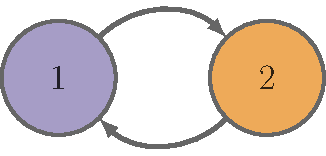
\includegraphics[width=2in]{projection.pdf}};

\node[text=textcolor] at (6,-6.5) {\LARGE \sffamily Restriction chains};
\node[inner sep=0pt] at (6,-9) {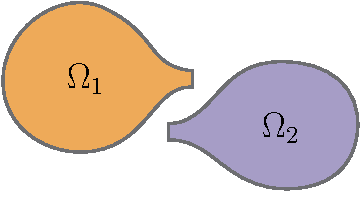
\includegraphics[width=2.5in]{restriction.pdf}};

\node[text=textcolor] at (-8,-11.5) {\LARGE \sffamily M\textsuperscript{3}\hspace{0.3em}--\hspace{0.4em}Lemma 4.5};
\node[text=textcolor] at (-8,-17.5) {\LARGE \sffamily Combined\hspace{0.4em}--\hspace{0.4em}Lemma 4.7};

\node[text=textcolor] at (6,-11.5) {\LARGE \sffamily Gibbs\hspace{0.4em}--\hspace{0.4em}Corollary 4.4 (Ding et al., 2009)};
\node[text=textcolor] at (6,-17.5) {\LARGE \sffamily Combined\hspace{0.4em}--\hspace{0.4em}Lemma 4.8};

\node[] (41) at (-8,-12.5) {};
\node[] (42) at (-8,-16.5) {};
\draw [-latex,line width=2.5pt,color=textcolor!60!white,line cap=round] (41) to[] (42);

\node[] (51) at (6,-12.5) {};
\node[] (52) at (6,-16.5) {};
\draw [-latex,line width=2.5pt,color=textcolor!60!white,line cap=round] (51) to[] (52);

\node[text=textcolor] at (-1,-14.5) {\LARGE \sffamily Comparison arguments (Diaconis \& Saloff-Coste, 1993)};

\node[] (6) at (-8, -18.5) {};
\node[] (7) at (6,-18.5) {};
\node[] (8) at (-1,-25.5) {};
\draw [-latex,line width=2.5pt,color=textcolor!60!white,line cap=round] (6) to[out=-90,in=90] (8);
\draw [-latex,line width=2.5pt,color=textcolor!60!white,line cap=round] (7) to[out=-90,in=90] (8);
\node[text=textcolor] at (-1,-21.5) {\LARGE \sffamily Theorem 4.9 (Jerrum et al., 2004)};

\node[text=textcolor] at (-1,-26.5) {\LARGE \sffamily Combined\hspace{0.4em}--\hspace{0.4em}Theorem 4.6};
\node[inner sep=0pt] at (-1,-29) {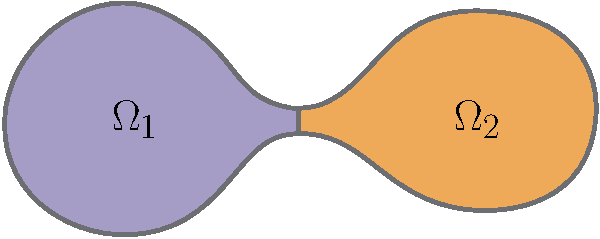
\includegraphics[width=4in]{bottleneck1.pdf}};
\end{tikzpicture}
\end{document}